%% Roman Link's personalized LaTeX Beamer template 
%% contact: rlink@gwdg.de

%% define document class and settings -----------------------------------
\documentclass[usepdftitle=false]{beamer}

%% fonts and input encoding ---------------------------------------------
\usepackage[T1]{fontenc}
\usepackage[utf8x]{inputenc}
\usepackage{lmodern}

%% language support -----------------------------------------------------
\usepackage[english]{babel} % english hyphenation etc.
\usepackage{babelbib}       % multi-language references

%% graphics and colors --------------------------------------------------
\usepackage{graphicx}  
\usepackage{color,pgf}
\usepackage{pdfpages}  % enables the use of pdf graphics

%% mathematical symbols  ------------------------------------------------
\usepackage{amsmath, amsfonts, amssymb, pgf}
\usepackage{eulervm}

%% references with natbib -----------------------------------------------
%\usepackage[round]{natbib}
%\def\newblock{} % hilft gegen absurde fehler mit natbib

%% tweaks of appearance -------------------------------------------------
\usepackage{subscript} % subscripts outside of math expressions
\usepackage{booktabs}  % better-looking tables
\usepackage{ragged2e}  % justified text in Beamer documents with  	
                       % \justifying{}
\usepackage{setspace}  % control line space with spacing environment

%% LaTeX Beamer settings ------------------------------------------------
\mode<presentation>{
	\usecolortheme{seahorse,rose}
	\useinnertheme[shadow]{rounded}
	% \useoutertheme[hideothersubsections,right,width=4em,frame  number]{sidebar}
	% \useoutertheme{infolines}
	% \useoutertheme{split}
	\useoutertheme[subsection=false,footline=authortitle]{miniframes}
	\setbeamercovered{transparent}
}

%% add slide numbers to all slides --------------------------------------
\addtobeamertemplate{navigation symbols}{
  {\usebeamercolor{section in toc}
   \footnotesize
   \insertframenumber/\inserttotalframenumber}
   \hspace{48em}
}{}

%% changes of beamer fonts ----------------------------------------------
\setbeamerfont{section in toc}{size=\normalsize,series=\bfseries}
\setbeamerfont{title}{series=\bfseries}
\setbeamerfont{frametitle}{size=\Large,series=\bfseries}

%% new LaTeX commands ---------------------------------------------------
\newcommand{\sub}[1]{\textsubscript{#1}}
\newcommand{\Sup}[1]{\textsuperscript{#1}}
\newcommand{\COO}{CO\textsubscript{2}}
\newcommand{\masl}{m~a.s.l.}
\newcommand{\gc}{$^{\circ}$C}
\newcommand{\tilt}{$\sim$}
\newcommand{\blue}[1]{{\color{blue!50!black}#1}}
\newcommand{\Blue}[1]{{\color{blue!50!black}\textbf{#1}}}
\newcommand{\eg}{e.\,g.}
\newcommand{\Eg}{E.\,g.}
\newcommand{\rar}{$\rightarrow$}
\newcommand{\lar}{$\leftarrow$}
\newcommand{\Rar}{$\Rightarrow$}
\newcommand{\Lar}{$\Leftarrow$}
\newcommand{\source}[1]{\baselineskip8pt{\tiny \color{gray} #1}}
\newcommand{\tw}{\textwidth}
\newcommand{\ddx}[2]{
	\frac{\mathrm{d}}{\mathrm{d}#2}#1 
	}
\newcommand{\ddxx}[2]{
	\frac{\mathrm{d^2}}{\mathrm{d}#2^2}#1
	}
\newcommand{\code}[1]{
	{\footnotesize 
	 \color{blue}
   \texttt{#1}}
   \normalsize
   \color{black}
  }

%% new environment for slides with changed margins ----------------------
\newenvironment{changemargin}[2]{%
	\begin{list}{}{%
			\setlength{\topsep}{0pt}%
			\setlength{\leftmargin}{#1}%
			\setlength{\rightmargin}{#2}%
			\setlength{\listparindent}{\parindent}%
			\setlength{\itemindent}{\parindent}%
			\setlength{\parsep}{\parskip}%
		}%
		\item[]}
	{\end{list}
}

%% pdf information  -----------------------------------------------------
\hypersetup{
	pdfauthor={Roman M. Link},
	pdftitle={Drought in tropical forests},
}

%% title page settings --------------------------------------------------
\title{Drought in tropical forests}
\subtitle{\normalfont The role of tree height and wood density for hydraulic efficiency, productivity and vulnerability to cavitation of trees along a lowland precipitation gradient}
\author[R. Link]{Roman Link}
\date{January 25, 2018}
\institute[University of Göttingen]{
Department of Plant Ecology and Ecosystem Research\\ Georg August University of Göttingen}
%\titlegraphic{ \vspace*{2em}
%\includegraphics[width=0.7\textwidth]{logouni.png}}
% logo - shown on all pages
\logo{\includegraphics[width=20em]{logo_uni_goe_transparent.png}}

%% start of document ----------------------------------------------------
\begin{document}

%% insert title page ----------------------------------------------------
\begin{frame}
\titlepage
\end{frame}

%% begin of regular slides ----------------------------------------------
\begin{frame}
	\frametitle{Structure of my PhD project}
	\begin{itemize}
		\item<+-| alert@+>  \Blue{Chapter 1:} Predicting radial sap flow profiles from Costa Rican tropical dry forest species
		\item<+-| alert@+>  \Blue{Chapter 2:} Estimating plant vulnerability to embolism in Costa Rican humid tropical forest species
		\item<+-| alert@+>  \Blue{Chapter 3:} Relationship between productivity, structural, functional, wood anatomical and hydraulic traits of tropical forest species from Costa Rica
		\item<visible@+-> \Blue{Bonus Chapter:} 
		\alert<5>{Maximum-likelihood estimation of xylem vessel lengths}\visible<6>{: \alert<6>{\textbf{Not in the focus of this presentation!}}
		}
    \end{itemize}	
\end{frame}

\section{Introduction}
\begin{frame}
	\frametitle{Introduction}
	\begin{itemize}
		\item Basics about plant water relations
		\item Why is it important to know about drought effects in the tropics?
	\end{itemize}
\end{frame}

\begin{frame}
	\frametitle{Main research questions}
	\begin{itemize}
		\item This one's gonna be tough
	\end{itemize}
\end{frame}

\begin{frame}
	\frametitle{Design of the study}
	\begin{minipage}{0.5\tw}
		\begin{itemize}[<+-| alert@+>]
			\item 5 research sites along a rainfall gradient on the Pacific shoreline of Costa Rica 			
			\item Gradient from tropical dry forest to humid tropical lowland forest
			\item Based on existing research sites of the \textbf{Instituto Tecnológico de Costa Rica}
		\end{itemize}		
	\end{minipage}
	\begin{minipage}{0.48\tw}
		\includegraphics[width = \tw]{figures/map_01_all_sites.png}  	
	\end{minipage}
\end{frame}

\begin{frame}
	\frametitle{Design of the study}
	\begin{minipage}{0.5\tw}
		\textbf{ At each of the 5 research sites:}
		\begin{itemize}[<+-| alert@+>]
			\item 8 species representing a gradient in tree height and wood density
			\item 5 replicates per species (only mature trees)
			\item[\Rar] 40 trees per site, 200 trees in total
		\end{itemize}	
	\end{minipage}
	\begin{minipage}{0.48\tw}
		\includegraphics[width = \tw]{figures/map_01_all_sites.png}  	
	\end{minipage}
\end{frame}


\begin{frame}
	\frametitle{Design of the study}
	\begin{itemize}
		\item \Blue{Variables measured at all sites}
		\begin{itemize}
			\item \alert<1>{Tree level}
			\begin{itemize}
				\item Diameter at breast height
				\item Tree height
				\item Tree growth (basal area/aboveground biomass increment)
				\item Wood density
				\item Sapwood non-structural carbohydrate (NSC) content
			\end{itemize}
			 \item  \alert<1>{Site level}
			  \begin{itemize}
			  	\item Temperature
			  	\item Relative humidity 
			  	\item Precipitation
			  \end{itemize}
		\end{itemize}		
		\item<2> \Blue{Variables measured at a subset of sites}
		\begin{itemize}
			\item  \alert<2>{Sap flow} (only at one site)
			\item  \alert<2>{Branch vulnerability to embolism} (only at two sites)
		\end{itemize}
	\end{itemize}
\end{frame}

\begin{frame}
	\frametitle{Problems with the design}
	\begin{itemize}
		\item<+-> \alert<1>{Opportunistic use of pre-existing plots}
		\begin{itemize}
			\item<+-| alert@+> Different plot sizes and numbers at each site
			\item<+-| alert@+> Differences in historic land use (pristine primary forest vs. disturbed primary forest vs. secondary forest)
			\item<+-| alert@+> Cooperation with forestry department (foresters do forester things...)
		\end{itemize}	
		\item<visible@+-| alert@+>[\rar] Plot-based comparisons are difficult
		\item<visible@+-| alert@+>[\Rar] Not that important for my (eco-physiological) research questions, but limits usability of plot network for other research areas
	\end{itemize}
\end{frame}


\section{Radial sap flow profiles}
\begin{frame}
	\frametitle{First chapter: radial sap flow profiles}
	\begin{minipage}{0.5\tw}
	 \textbf{Sap flow measurements:}
	 \begin{itemize}
	 	\item<+-| alert@+> Practical limitations \rar\ only in dry forest (Horizontes)
	 	\item<+-| alert@+> 4 measurement campaigns of $\pm$ 1 week during rainy season of 2015
	 	\item<+-| alert@+> 40 trees of 8 species	
	 	\item<+-| alert@+> Measured with the Heat Field Deformation (HFD) method			
	 \end{itemize}			
	\end{minipage}
	\begin{minipage}{0.48\tw}
		\only<1>{\includegraphics[width = \tw]{figures/map_02_horizontes.png}} 	
		\only<2-3>{\includegraphics[width = \tw]{figures/Guanacaste2015.jpg}\\
			
			\source{Image source: Instituto Meteorológico Nacional de Costa Rica}} 			
		\only<4>{\centering 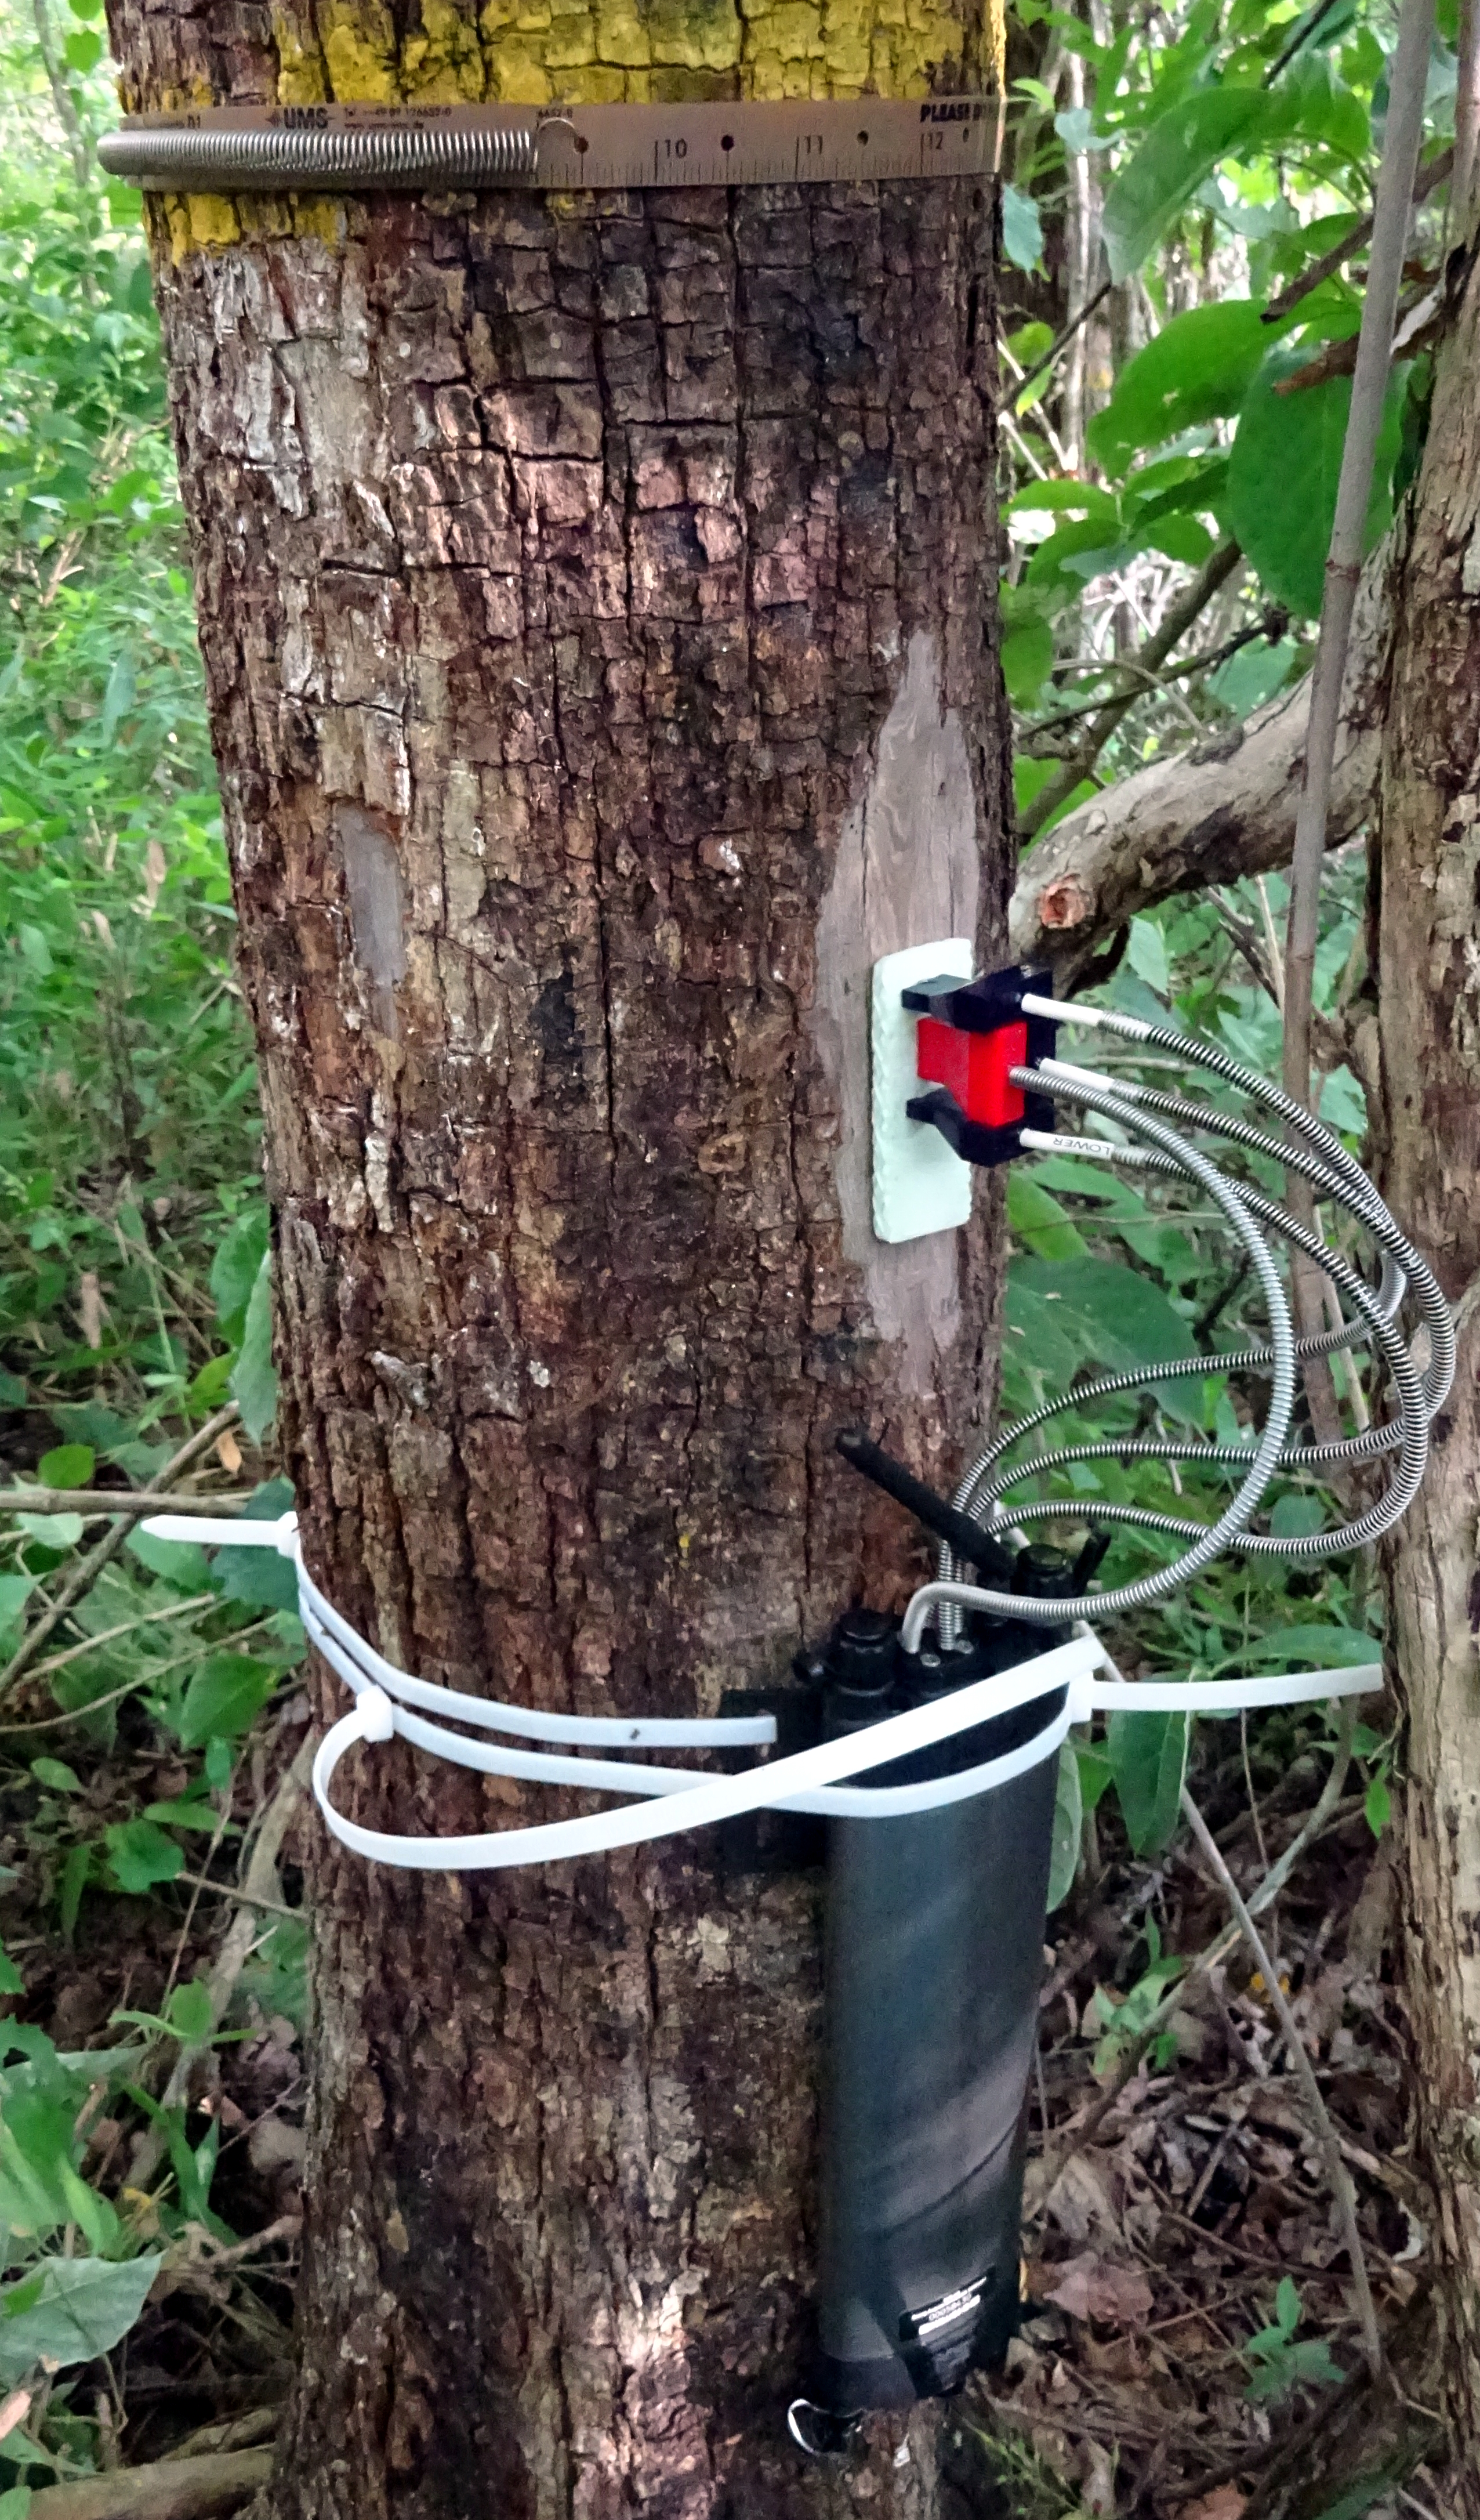
\includegraphics[width = 0.7\tw]{figures/HFD_01_sensor.JPG}}
	\end{minipage}
\end{frame}

\begin{frame}	
	\includegraphics[height = \textheight]{figures/horizontes_WD_height1.png}
\end{frame}

\begin{frame}
	\frametitle{First chapter: radial sap flow profiles}
  \Blue{Additionally measured:}
  \begin{itemize}
  	\item \alert{Soil water content}
  	\begin{itemize}
  		\item 1 measurement for each of the 4 campaign
  		\item 1 soil sample per subplot ($4\times45$ in total)
  	\end{itemize}
  	\item \alert{Vertical microclimate}
  	\begin{itemize}
  		\item Temperature + air humidity tracked with \textit{iButtons}
  		\item Measured from ground level to canopy in 5~m steps
  		\item 3 measurement lines
  	\end{itemize}
  \end{itemize}
\end{frame}

\begin{frame}
	\frametitle{Heat field deformation sensors}
	\begin{minipage}{0.5\tw}
		\textbf{Working principle:}
		\begin{itemize}
			\item<+-| alert@+> 1 heater and 3 temperature sensors inserted into wood
			\item<+-| alert@+> Heater heats constantly with known caloric input
			\item<+-| alert@+> Sap movement \rar\ faster heat transport in flow direction
			\item<+-| alert@+> Temperature differences between sensors are used for estimation of sap flux density at different depths
		\end{itemize}						
	\end{minipage}
	\begin{minipage}{0.48\tw}
			\only<1-2>{\includegraphics[width = \tw]{figures/nadezhdina_01.png}}
			\only<3-4>{\quad\quad \includegraphics[width = 0.6\tw]{figures/nadezhdina_02.png}}\\
				
				\source{Image source: Nadezhdina et al., 2012}
	\end{minipage}
\end{frame}

\begin{frame}[t]
	\frametitle{Heat field deformation sensors}
	\begin{itemize}
		\item<only@1| alert@1> Original idea: comparison of sap flow and plant water use between species with different trait combinations
		\item<only@2-> Problem: newer research indicates that
		\begin{itemize}
			\item[a)]<2-| alert@2> The mechanistic explanation of the HFD method (Nadezhdina et al., 2012) is flawed (Vandegehuchte \& Steppe, 2012)\\ \rar\ species-specific calibration likely necessary in most cases
			\item[b)]<3-| alert@3-4> HFD calibration parameters are not consistent within species (Fuchs et al., 2017)
		\end{itemize}	
		\item<only@5-| alert@5>\textit{ Relative values} are probably reliable, \textit{absolute values} have to be handled with care
		\item<only@6| alert@6>[\Rar] \textbf{Decision for analysis: better to put focus on radial gradients of sap flux}
	\end{itemize}
	\only<2>{\includegraphics[width = \tw]{figures/vandegehuchte_01.png}}
  \only<3>{\includegraphics[width = \tw]{figures/HFDSeb_01_paper.png}}
  \only<4>{\centering \includegraphics[width = 0.45\tw]{figures/HFDSeb_02_accuracy.png}}		
\end{frame}

\begin{frame}
	\frametitle{Research questions \& hypotheses}
	\begin{minipage}{0.38\tw}
		\includegraphics[width = \tw]{figures/HFD_05_profile_simarouba.png}
	\end{minipage}
	\begin{minipage}{0.6\tw}
			\begin{itemize}
			\item Radial sap flow gradients
			\begin{itemize}[<+-| alert@+>]
				\item very important for studies of plant water use
				\item few methods take them into account
				\item sensors are expensive and error-prone
			  \item species specific measurement: problematic in the tropics		
			\end{itemize}
			\item<+-| alert@+>[\Rar] \Blue{Question:} Is it possible to predict the shape of radial sap flow profiles based on tree traits?
			\item<visible@+| alert@+>[\Rar] \Blue{Hypothesis:} The shape of radial sap flow profiles depends on \textbf{wood density} and \textbf{tree height}
		\end{itemize}						
	\end{minipage}
\end{frame}

\begin{frame}
	\frametitle{Data analysis}
	\begin{minipage}{0.38\tw}
		\includegraphics[width = \tw]{figures/HFD_05_profile_simarouba.png}
	\end{minipage}
	\begin{minipage}{0.6\tw}		
		   \Blue{How to analyze?}		
		\begin{itemize}[<+-| alert@+>]			
			\item Nonlinear relationship
			\item Parameters that control the shape of the nonlinear relationship depend on other variables
			\item Hierarchical data structure (repeated observations in replicate trees from different species)					
		\end{itemize}
	\end{minipage}
\end{frame}

\begin{frame}[t]
	\frametitle{Data analysis}
	\begin{itemize}
		\item Analysis based on \Blue{Bayesian nonlinear hierarchical models}
		\begin{itemize}			
			\item<2-> \alert<2>{\textbf{First stage of the model:}} Nonlinear relationship between sensor depth and predicted flux density modeled with the density function of the Weibull distribution
			\item<4->  \alert<4>{\textbf{Second stage of the model:}} Parameters of the Weibull distribution modeled as a function of wood density, tree height and their interaction, accounting for species and stem specific random variation
			\item<only@5->  \alert<5>{Model fitting with the \textbf{Stan modeling language}}
		\end{itemize}
		\item<only@6| alert@6> Models still need tuning \rar\ shown results are from preliminary model based on R package \texttt{nlme}
	\end{itemize}
	  \only<3-4>{\includegraphics[width = 0.8\tw]{figures/weibulldens.png}}
\end{frame}

\begin{frame}
	\frametitle{Model equations of the preliminary model}
  \includegraphics[height=0.9\textheight]{figures/HFD_06_model.png}
\end{frame}

\begin{frame}
	\includegraphics[height=\textheight]{figures/HFD_02_profiles.png}
\end{frame}

\begin{frame}
	\frametitle{Preliminary results I - predicted profiles}	
	\begin{minipage}{0.6\tw}
		\begin{itemize}[<+-| alert@+>]
			\item Model explains a large part of the observed variance in the dataset (conditional pseudo-R\Sup{2} = 0.918)
			\item Most of this variance is explained by random differences between species and stems (marginal pseudo-R\Sup{2} = 0.329)
		\end{itemize}						
	\end{minipage}
	\begin{minipage}{0.38\tw}
		\includegraphics[width = \tw]{figures/HFD_05_profile_simarouba.png}
	\end{minipage}	
\end{frame}

\begin{frame}[t]
	\frametitle{Preliminary results II - parameter model for K}
		\only<1>{\includegraphics[width=\tw]{figures/weibulldens_K.png}}
		\only<2>{\includegraphics[width=\tw]{figures/HFD_03a_k_responses.png}}
		\begin{itemize}
		\item \Blue{Weibull shape parameter K} 
			\begin{itemize}							
				\item<visible@2>	No significant height- and wood density effects
			\end{itemize}
	\end{itemize}
\end{frame}

\begin{frame}[t]
	\frametitle{Preliminary results II - parameter model for $\lambda$}
	\only<1>{\includegraphics[width=\tw]{figures/weibulldens_lambda.png}}
  \only<2>{\includegraphics[width=\tw]{figures/HFD_03b_lambda_responses.png}}
	\begin{itemize}
		\item \Blue{Weibull scale parameter $\lambda$}
		\begin{itemize}
			\item<visible@2> Decreases significantly with tree height and wood density, but significantly less so in trees that are both large AND have hard wood
		\end{itemize}	
	\end{itemize}
\end{frame}

\begin{frame}
	\frametitle{Radial sap flow profiles - Conclusions}
	\begin{itemize}[<+-| alert@+>]
		\item Shape of the profile significantly depends on height and wood density
		\item Model describes observed radial profiles very well
		\item Explained variance is much lower when predicting onto new trees because of the high stem-specific variability
		\item Inclusion of other predictors might improve predictions (and consequently increase the value of the model for studies of plant water use)
	\end{itemize}
\end{frame}


\section{Vulnerability curves}
\begin{frame}
	\frametitle{Second chapter: vulnerability curves}
	\begin{changemargin}{-1em}{-1em}	
		\centering{
			\includegraphics[width=0.65\tw]{figures/schuldt_2015_VC.png}}
		\begin{itemize}
			\item<only@1> \alert{Vulnerability curves:} relationship between \alert{water potential} and \alert{percentage loss of conductivity} (PLC)
			\item<only@1>[\rar] curve describes the loss of conductive function under increasingly dry conditions
			\item<only@2> \alert{Parameters of vulnerability curves:} important predictors of drought response
			\begin{itemize}
				\item  \Blue{P\sub{50}:} At what pressure 
				does a plant lose 50\% of its conductivity?  
				\item \Blue{Slope:} How fast does this loss occur?
			\end{itemize}
		\end{itemize}  
		\only<2>{\vspace{0.65em}}
		\source{Image source: Schuldt et al., 2016}
	\end{changemargin}	
\end{frame}

\begin{frame}
	\frametitle{Second chapter: vulnerability curves}
	\begin{minipage}{0.5\tw}
			\begin{itemize}
			\item<1-| alert@1> Vulnerability curves of replicate samples from 30 trees of 10 tropical forest species from the Osa peninsula (56 in total)
			\item<2-| alert@2-4> Collection of upper canopy branches in two campaigns in the rainy seasons  of 2016 and 2017
			\item<5-| alert@5-> Measured with the Cavitron method using a novel 1~m rotor (courtesy of the lab of Sylvain Delzon, Bordeaux) 
		\end{itemize}			
	\end{minipage}
	\begin{minipage}{0.48\tw}
		\centering
		\only<1>{\includegraphics[width = \tw]{figures/map_03_osa.png}}	
		\only<2>{\includegraphics[width = 0.75\tw]{figures/field1.jpg}}	
		\only<3>{\includegraphics[width = 0.75\tw]{figures/field2.jpg}}
		\only<4>{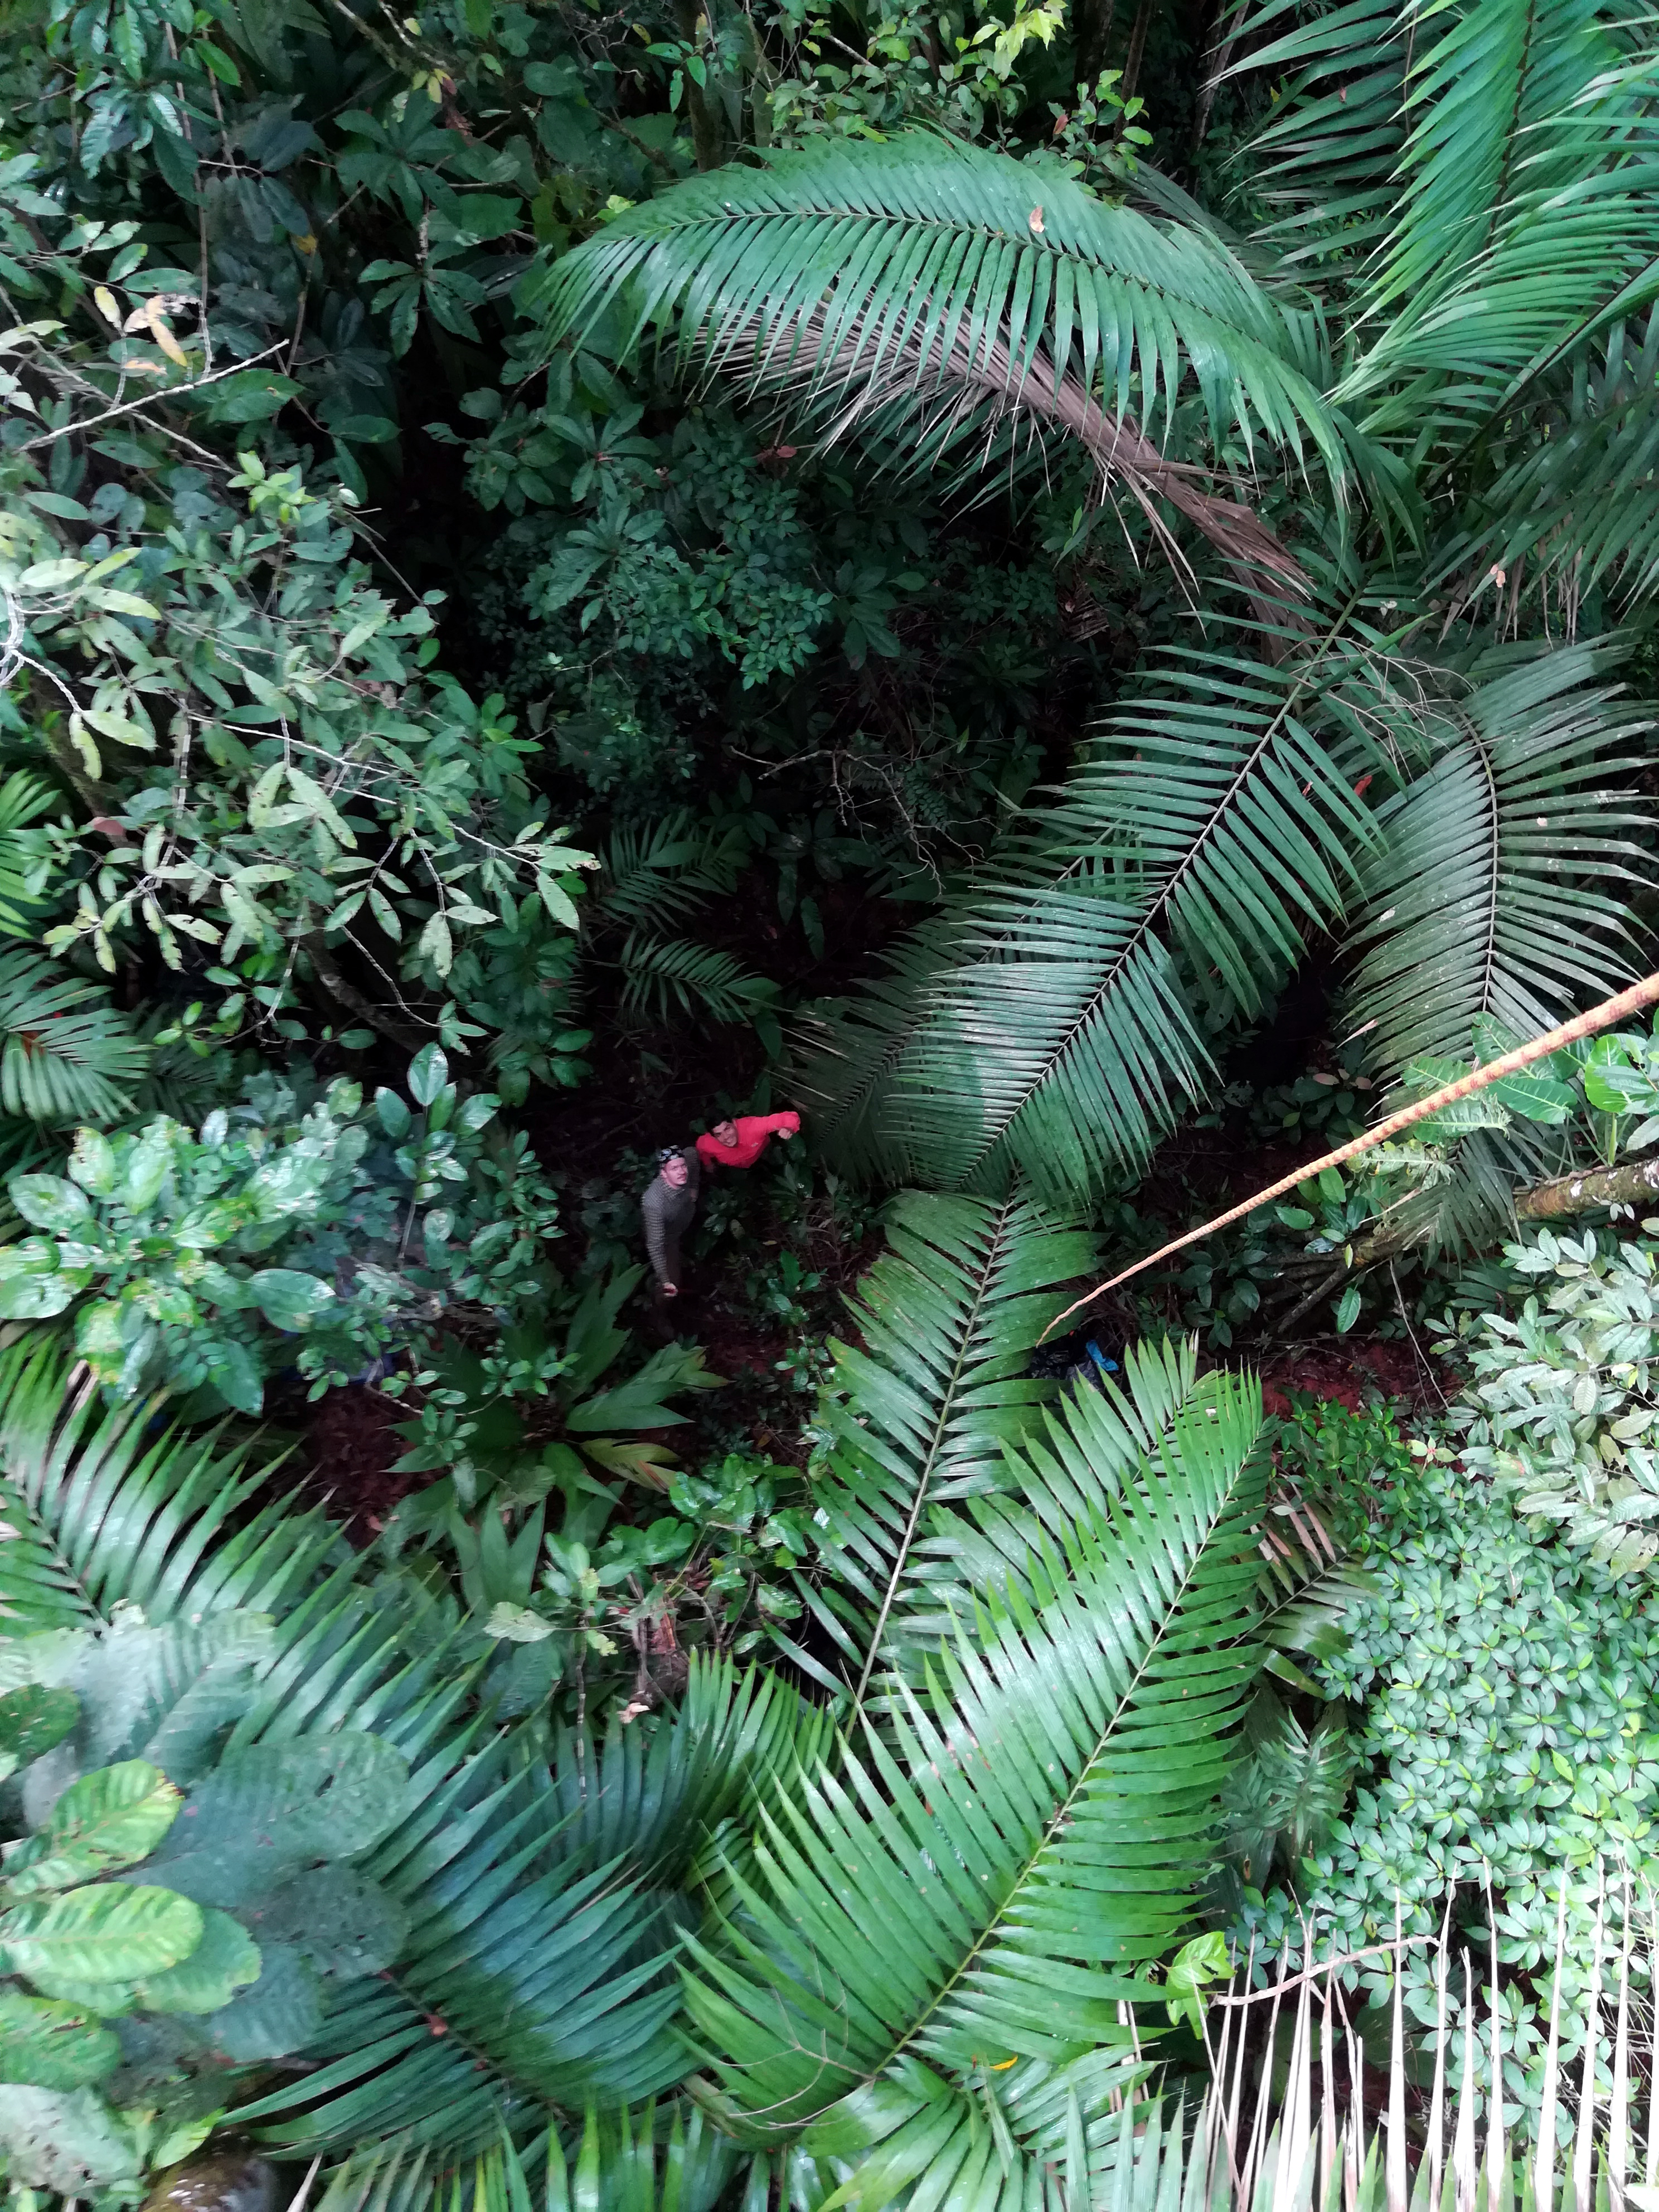
\includegraphics[width = 0.8\tw]{figures/field3.jpg}}
		\only<5>{\includegraphics[width = \tw]{figures/cavi01.jpg}\\			
			\source{Foto: \url{http://sylvain-delzon.com/caviplace/}}}
		\only<6>{\includegraphics[width = 0.9\tw]{figures/cavi02.jpg}\\
			\source{Foto: \url{http://sylvain-delzon.com/caviplace/}}}
		\end{minipage}	
\end{frame}


\begin{frame}
	\frametitle{Second chapter: vulnerability curves}
	\Blue{Additionally measured for each tree:}
	\begin{itemize}
		\item Maximum vessel length (1 per tree)
		\item Leaf nutrient contents (1 per sample)
		\item Specific leaf area (1 per sample)
		\item Anatomy of branch wood  (2 per sample)
		\item Huber value  (1 per sample)
		\item Branch non-structural carbohydrate storage  (1 per tree)
	\end{itemize}
\end{frame}



\begin{frame}
  \begin{block}{\textbf{Hypothesis}}
  The parameters of vulnerability curves are significantly related to plant structural, functional and wood anatomical traits:
  \begin{itemize}
  	\item Tree size (height and diameter)
  	\item Wood density
  	\item Vessel diameter \& vessel density
  \end{itemize}
  \end{block}
\end{frame}

\begin{frame}
	\frametitle{Data analysis}
	\centering{\includegraphics[width=0.38\tw]{figures/schuldt_2015_VC.png}}
	\begin{itemize}[<+-| alert@+>]
		\item Nonlinear relationship
		\item Parameters that control the shape of the nonlinear relationship (P50 and slope) depend on other variables
		\item Hierarchical data structure (repeated observations on replicate samples from replicate trees belonging to different species)		
		\item<visible@4-| alert@4>[\Rar] \textbf{Nonlinear hierarchical models}\\ (analogous to models for radial sap flow profiles)
		\item<visible@5| alert@5>[\Rar] \textbf{\Large Data analysis in progress}
	\end{itemize}	
	\source{Image source: Schuldt et al., 2016}
\end{frame}

\begin{frame}
	\frametitle{Observed vulnerability curves}
		\includegraphics[height=0.9\textheight]{figures/VC_02_preliminary_plot.jpg}
\end{frame}

\section{The big picture}
\begin{frame}
	\begin{block}{\textbf{Third chapter: moving on to the big picture}}
		\begin{itemize}
			\item Do structural, functional and wood anatomical traits explain changes in productivity and hydraulic traits observed along the rainfall gradient? 
			\item How are they related to non-structural carbohydrate storage?
		\end{itemize}
	\end{block}	
\end{frame}

\begin{frame}
	\frametitle{Synthesizing the results of the gradient study}	\Blue{Variables that are relevant for the synthesis}
	\begin{itemize}[<+-| alert@+>]
		\item Tree size (tree height + diameter at breast height)
		\item Wood density
		\item Wood anatomy (average vessel diameter, vessel density, potential hydraulic conductivity)
		\item Wood non-structural carbohydrate contents
		\item Productivity (basal area increment/aboveground biomass increment)
		\item Climate information (?)
		\item<visible@+| alert@+> \textbf{Sap flow data and vulnerability curves: unfortunately not available for all sites}		
	\end{itemize}	
\end{frame}

\begin{frame}
	\frametitle{Research questions \& hypotheses}
	\begin{changemargin}{-2em}{-2em}
		\Blue{Hypotheses from the project proposal related to these variables}
		\begin{itemize}
			\item \alert<1>{\textbf{Productivity}}
			\begin{itemize}
				\item increases with potential hydraulic conductivity
				\item is related to tree height
				\item is related to wood density (only at seasonally dry sites)
			\end{itemize}
			\item<2-> \alert<2>{\textbf{Potential hydraulic conductivity}}
			\begin{itemize}
				\item increases with tree height
			\end{itemize}
			\item<3-> \alert<3>{\textbf{Average vessel diameter}}
			\begin{itemize}
				\item increases with tree height (in trunk and branches)
			\end{itemize}
			\item<4-> \alert<4>{\textbf{NSC storage}}
			\begin{itemize}
				\item increases with tree size
				\item is higher at seasonally dry sites
				\item is higher in deciduous trees/trees with isohydric drought response
			\end{itemize}
		\end{itemize}
	\end{changemargin}
\end{frame}

\begin{frame}
	\frametitle{Data analysis}
	\begin{itemize}
		\item<+-| alert@+> Large amount of interrelated causal hypotheses about relationships between variables
		\item<+-| alert@+>[\Rar] Instead of focusing on the bivariate relationships in our system one at a time, test them all at once
		\item<visible@+-| alert@+>[\Rar]\textbf{Structural equation modeling}
		\begin{itemize}
			\item Modeling framework for the multivariate analysis of networks of causal hypotheses
			\item Allows to test whether a system significantly deviates from a model based on a-priori hypotheses about the system
		\end{itemize}		
	\end{itemize}
\end{frame}

\begin{frame}
	\frametitle{Data analysis}
	\begin{itemize}
		\item Dataset is not complete (NSC data are being measured)
		\item<2-> To show what the analysis will look like - results from a study using an analogous model:\\
		
		\vspace{1em} \blue{Kotowska, M.M., Röll, A., \alert{Link, R.M.,} Hertel, D., Hölscher, D., Leuschner, C., Waite, P.A., Moser, G., Toja, A, Schuldt, B. (2018):} \textit{Tree size in combination with wood anatomy determines whole-tree water use and productivity in the tropics} (in preparation)		
		
	\end{itemize}
\end{frame}



\begin{frame}
	\frametitle{Meta-model}
	\begin{changemargin}{-2em}{-2em}
		\centering
		\only<1>{\includegraphics[height = 0.52\textheight]{figures/SEMartyna_01_metamodel.png}}
		\only<2->{\includegraphics[height = 0.52\textheight]{figures/SEMartyna_02_metamodel1.png}}
		\begin{itemize}
			\item<alert@1> \textbf{Meta-model:} relationships between theoretical entities/constructs of interest
			\item<2-| alert@2> Updated because to reflect the different effects of the components of both tree size and sap flow
			\item<visible@3| alert@3> For our model: remove sap flow component, add component for NSC
		\end{itemize}
	\end{changemargin}
\end{frame}

\begin{frame}
	\frametitle{Causal diagram}
	\begin{changemargin}{-2em}{-2em}
		\centering
	\includegraphics[height = 0.6\textheight]{figures/SEMartyna_03_causal_diagram.png}
		\begin{itemize}
			\item<alert@1> \textbf{Causal diagram:} Representation of the variables in the model and the assumed causal links
			\item<2-| alert@2> Blue arrows: links related to a priori hypotheses
		\end{itemize}
	\end{changemargin}
\end{frame}

\begin{frame}
	\frametitle{Path diagram of final model}
	\centering
	\includegraphics[height = 0.65\textheight]{figures/SEMartyna_04_path_diagram.png}
	\begin{itemize}[<+-| alert@+>]
		\item $\chi$² = 3.35, df = 7, p = 0.850; CFI = 1.00, RMSEA = 0.00
		\item Links were removed when related to tests of a priori hypotheses that were not significant 
	\end{itemize}
\end{frame}

\begin{frame}
	\frametitle{Summary: current state of the project}	
	\begin{itemize}
		\item<1-> \Blue{Chapter 1: radial sap flow profiles}
		\begin{itemize}
			\item Dataset complete
			\item Preliminary results: shape of radial profiles significantly predicted by wood density and tree height, but effect minute compared to random stem differences 
			\item \textbf{Current state: \alert<1>{data analysis}}
		\end{itemize}
		\item<2-> \Blue{Chapter 2: Vulnerability curves}
		\begin{itemize}
			\item Leaf nutrient contents, branch NSC and branch anatomy missing
			\item \textbf{Current state: \alert<2>{waiting for data}}
		\end{itemize}
		\item<3-> \Blue{Chapter 3: Structural equation models}
		\begin{itemize}
			\item NSC dataset missing
			\item \textbf{Current state: \alert<3>{waiting for data}}
		\end{itemize}
		\item<4-> \Blue{Bonus chapter: Vessel lengths}
		\begin{itemize}
			\item \textbf{Current state: \alert<4>{submitted}}
		\end{itemize}
	\end{itemize}
\end{frame}

	\begin{frame}[plain]
		\begin{block}{\textbf{Thanks list (in mostly alphabetical order):}}
			Dagoberto Arias, Marvin Castillo, Sylvain Delzon, Adrian Fröhlich, Sebastian Fuchs, Steven Jansen, Christoph Leuschner, Erick Naranjo, Maynor Rodriguez, Luis Guillermo Romero, Bernhard Schuldt, Katja Steinhoff, Juan Carlos Valverde, the CIPA staff, the EEFH staff, the Escuela de Ingiería Forestal of the TEC, and everyone who feels forgotten
		\end{block}		
	\end{frame}


{
	\usebackgroundtemplate{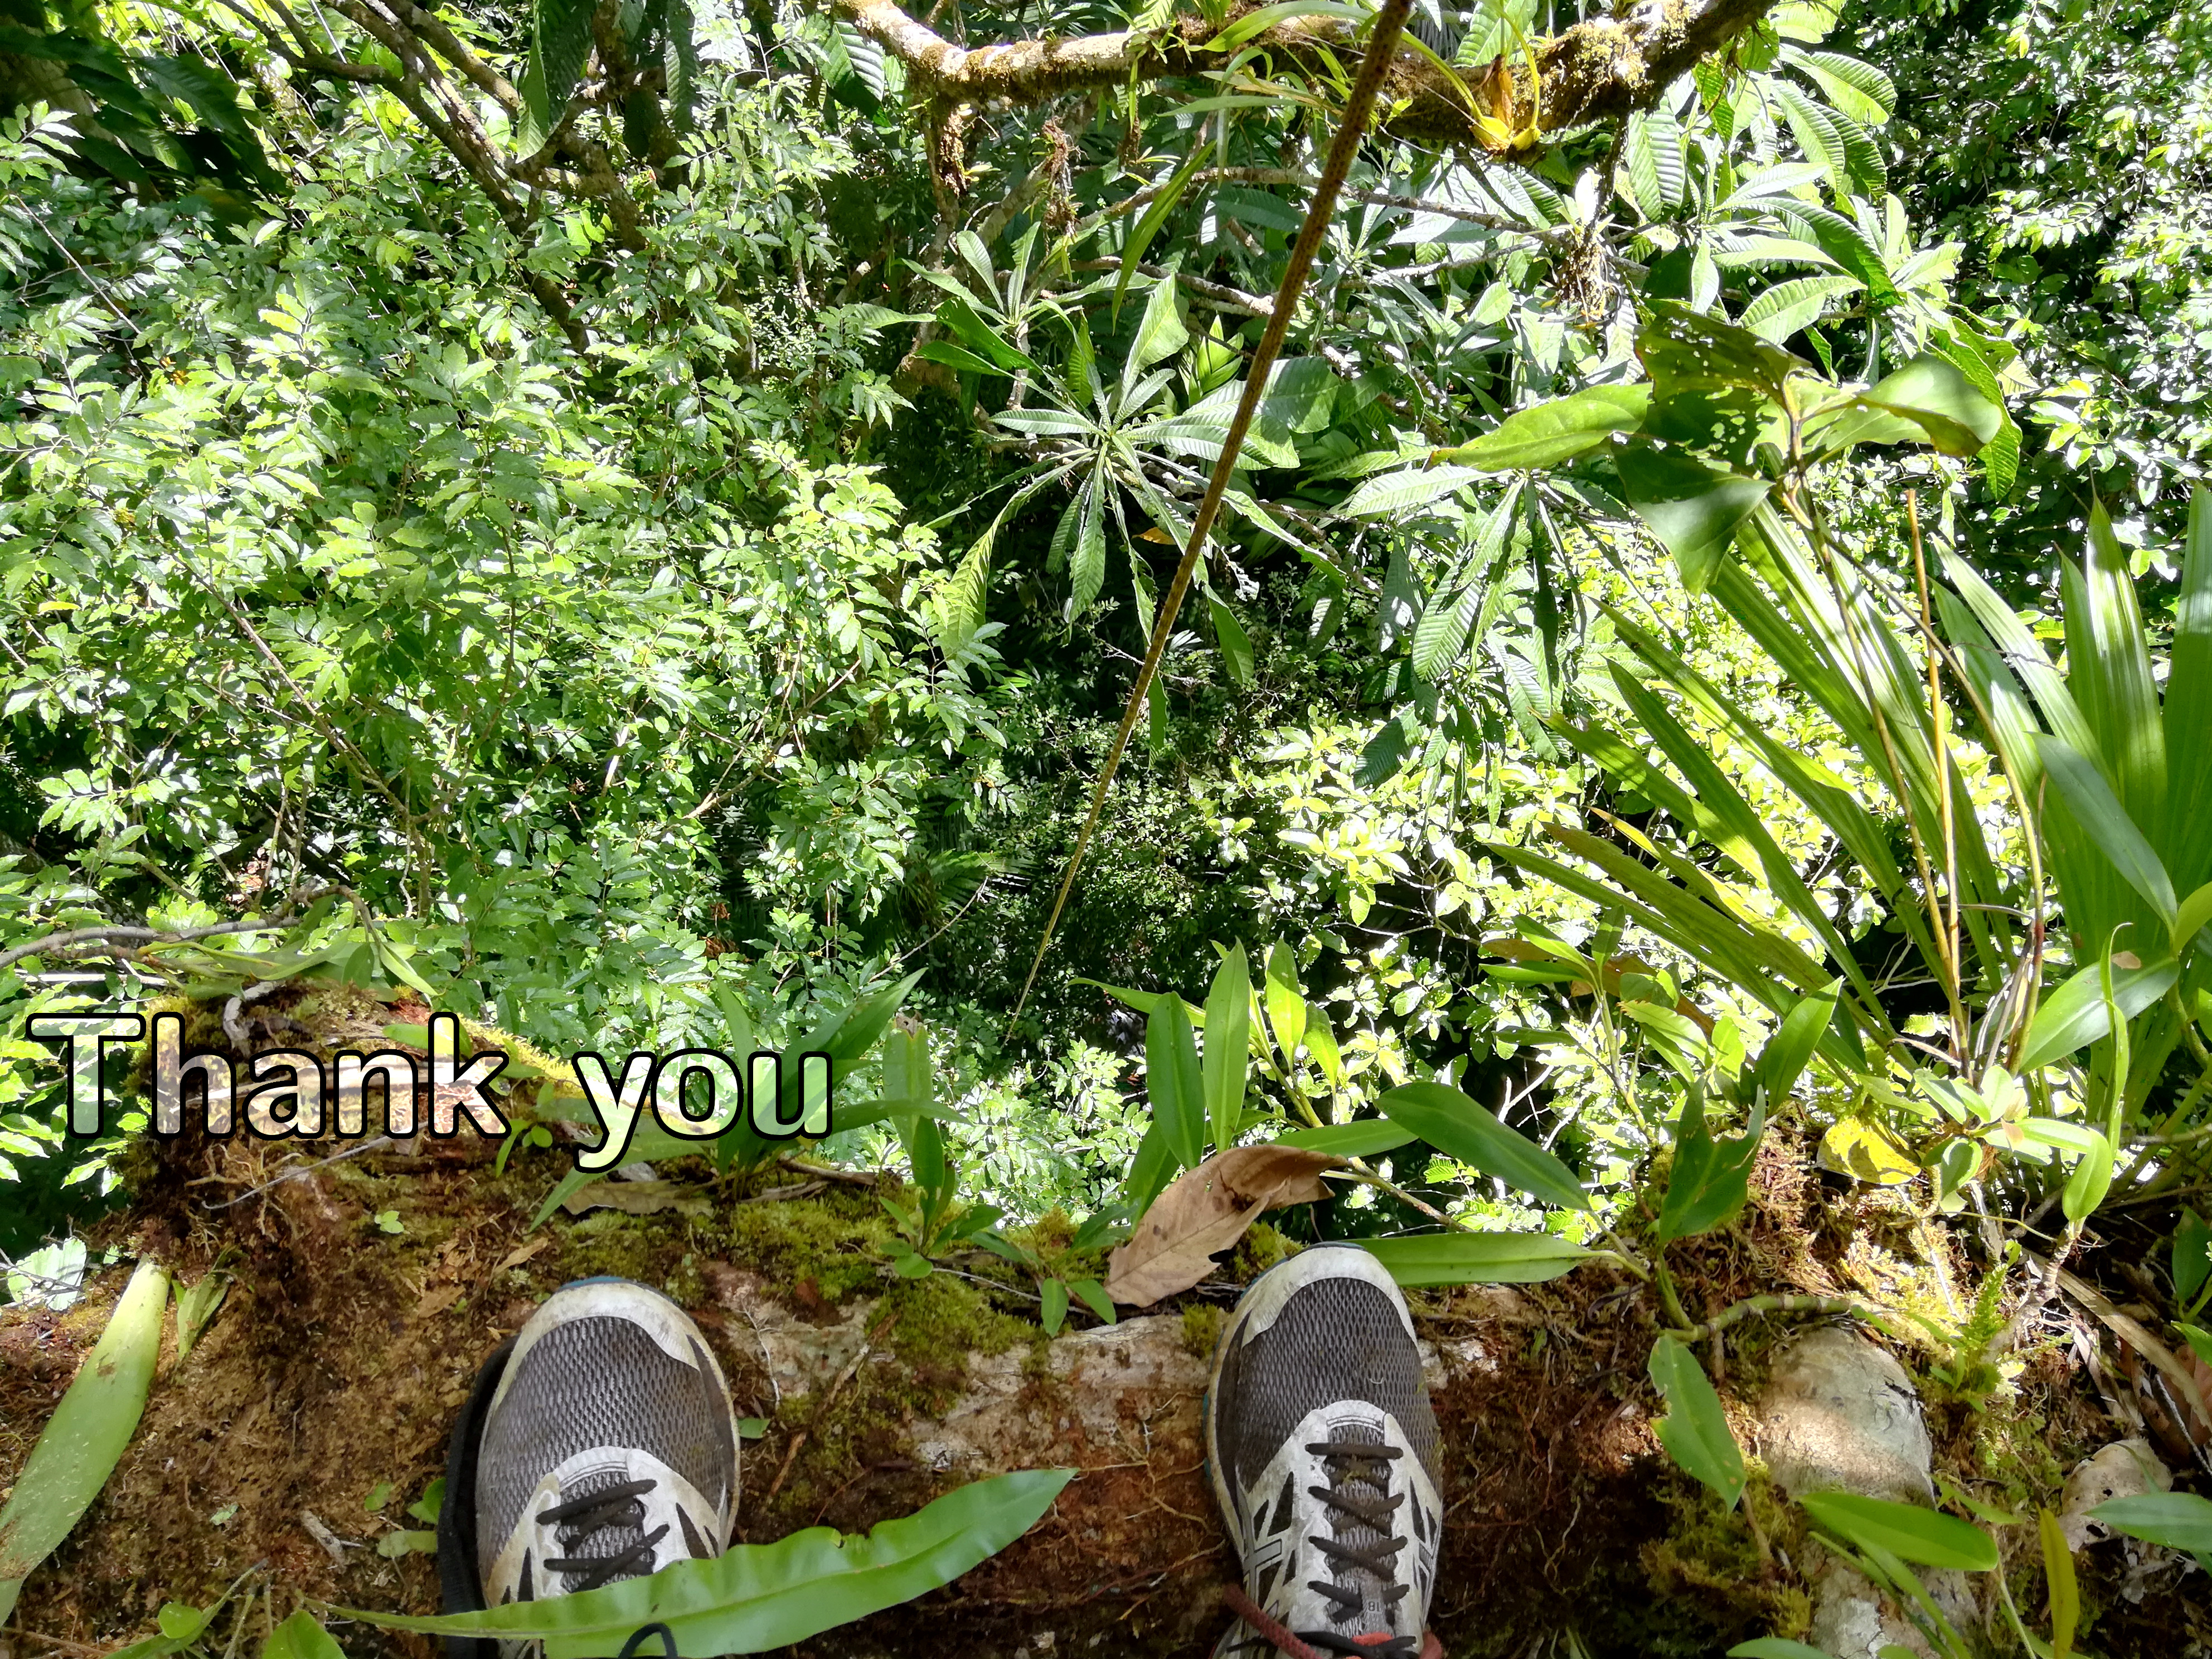
\includegraphics[height=\paperheight,width=\paperwidth]{figures/thankyou.jpg}}
	\setbeamertemplate{navigation symbols}{}
	\begin{frame}[plain]
	\end{frame}
}

\section{References}
\begin{frame}[t]
	\frametitle{References}
	\begin{changemargin}{-2em}{-2em}
		\footnotesize
		\begin{itemize}
			\item \textbf{Fuchs S, Leuschner C, Link R, Coners H, Schuldt B, 2017.}
			Calibration and comparison of thermal dissipation, heat ratio and heat field deformation sap flow probes for diffuse-porous trees,
			\textit{Agricultural and Forest Meteorology} \textbf{244–245}, 151-161. \url{https://doi.org/10.1016/j.agrformet.2017.04.003}.
			\item \textbf{Nadezhdina, N, Vandegehuchte, MW, Steppe, K, 2012.} Sap flux density measurements based on the heat field deformation method. \textit{Trees} \textbf{26(5)}, 1439-1448.
			\item \textbf{Schuldt B, Knutzen F, Delzon S, Jansen S, Müller-Haubold H, Burlett R, Clough, Y, Leuschner, C, 2016.} How adaptable is the hydraulic system of European beech in the face of climate change-related precipitation reduction?. \textit{New Phytologist} \textbf{210(2)}, 443-458.
			\item \textbf{Vandegehuchte, MW,  Steppe, K, 2012.} Interpreting the Heat Field Deformation method: Erroneous use of thermal diffusivity and improved correlation between temperature ratio and sap flux density. \textit{Agricultural and Forest Meteorology} \textbf{162}, 91-97.
		\end{itemize}
	\end{changemargin}
\end{frame}
\end{document}
